\documentclass{article}

\usepackage[english, russian]{babel}
\usepackage{amsmath}
\newcommand{\Mod}[1]{\ (\mathrm{mod}\ #1)}
\usepackage[letterpaper,top=2cm,bottom=2cm,left=3cm,right=3cm,marginparwidth=1.75cm]{geometry}
\usepackage[usenames,dvipsnames]{color}
\usepackage{caption}

\setlength{\abovedisplayskip}{3pt}
\setlength{\abovedisplayshortskip}{3pt}
\setlength{\belowdisplayskip}{3pt}
\setlength{\belowdisplayshortskip}{3pt}
\usepackage[14pt]{extsizes} 

\DeclareMathAlphabet{\pazocal}{OMS}{zplm}{m}{n}
\newcommand{\unif}{\pazocal{U}}

\linespread{1.6}

\usepackage{amsmath}
\usepackage{graphicx}
\usepackage[colorlinks=true, allcolors=blue]{hyperref}
\usepackage{fancyvrb} % for "\Verb" macro
\VerbatimFootnotes    % enable use of \Verb in footnotes

\title{Генерация данных}
\date{}
\begin{document}
\maketitle

\section*{Введение}
Первым шагом на пути к решению задачи является поиск/генерация данных для дальнейшего обучения, тестов, проверок гипотез.

Чем данные будут более правдоподобные, тем точнее можно будет сказать о том, получается ли решать задачу, какой из подходов работает лучше и прочее. В процессе разработки генератор скорее всего будет дорабатываться и, главеное, расширяться, становясь более правдоподобным.

Нужно сделать так, чтобы на выходе могли получаться реалистичные и разнообразные данные. Разнообразие здесь важно, так как, если будет много типичных данных, то модель будет сильно переобучаться, или находить паттерны, не подходяшие для решения задачи в общем случае.

Решено было разделить задачу на два этапа: создание генератора искусственных данных и создание функционала для получения (через апи или парсинг) реальных данных из каких-то источников.

\section*{Искусственный генератор данных}
Для создания искусственного генератора данных использовалсь библиотека Faker. Она содержит в себе много провайдеров, генераторов для создания правдоподобных случайных данных.

Для того, чтобы в полной мере воспользоваться возможностями Faker и сделать данные более разнообразными, при генерации используются все (за исключением некоторых, например генератора csv или json) возможные методы генерации случайных данных. 

В разработанный класс подается число таблиц $N$, которые нужно снегерировать, специфицируется язык для генерации контента (например, имен и городов, а также локализация учитывает специфичные особенности выбранного региона (это от самого функционала Faker)), диапазон в котором генерируются число столбцов (каждый раз случайно для каждой таблицы), и диапазон количества строк. Итогом гереации является $N$ сгенерированных .csv файлов, разнообразных настолько, насколько это позволяет функционал Faker.

Для исходной задачи создается два генератора, один для генерации в русской локализации, другой для генерации в английской.

\begin{figure}[hbt!]
\centering
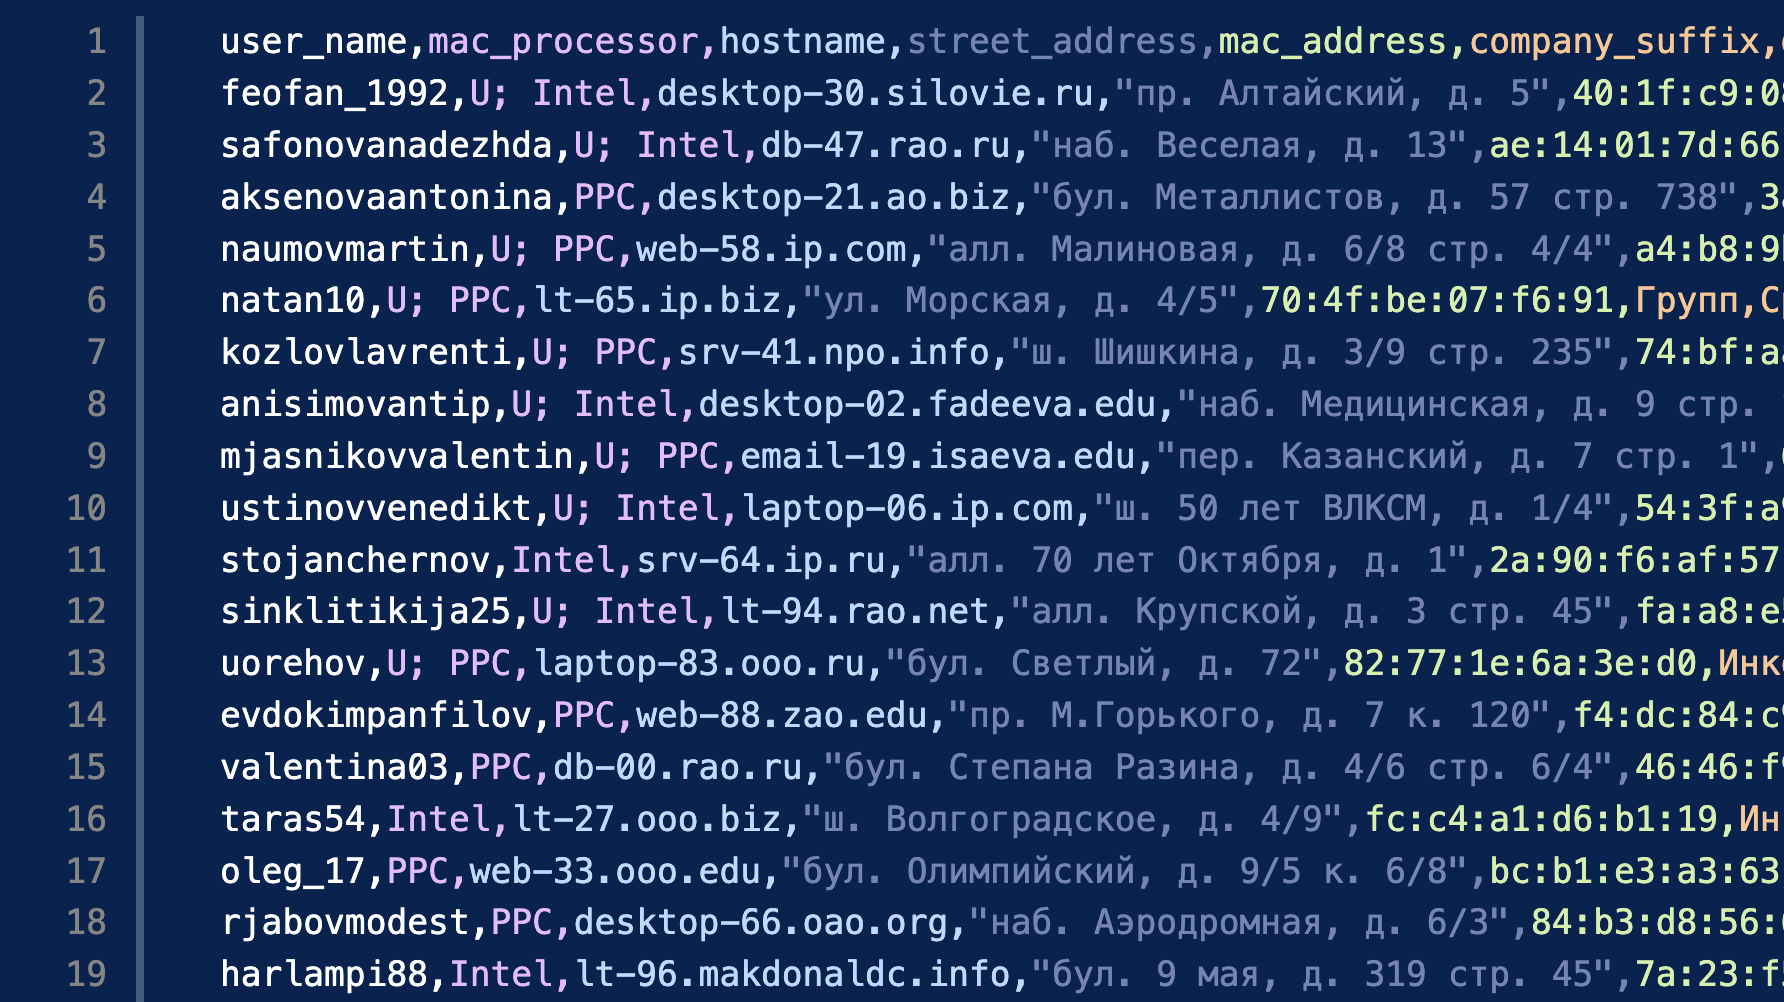
\includegraphics[width=0.8\linewidth]{figures/generated_data_example.png}
\captionof{figure}{Пример сгенерированных данных.}
\end{figure}

\section*{Использование реальных наборов данных}
Так или иначе, функционал Faker ограничен, для расширения наборов данных было решено использовать общедоступные реальные датасеты.

Для поиска наборов данных использовалась платформа Kaggle, взаимодействие с которой велось через kaggle-api в Python.

По итогу разработан класс, который во-первых скачивает выбранное количество датасетов с использованием заранее заданных поисковых запросов (и фильтров на размер датасета и его типа (ищутся .csv)), а во-вторых совершает случайные запросы, и также скачивает, и распаковывает датасеты. Для каждого запроса он скачивает выбранное число датасетов (чтобы были схожие по тематике, но разные по данным наборы).

\section*{Заключение}
По итогу, было использовано два разных подхода к получению данных. Первый, это генерация искусственных данных, такой подход может быть менее разнообразным, но его можно бесконечно расширять под разные реалии. Так, легко и гибко можно добавить самописный провайдер, который будет генерировать нужные нам, специфичные данные.

Второй подход, это использование реальных наборов данных. Такой подход менее контролируемый, но позволяет получать более разнообразные данные.
\end{document}